\documentclass[12pt]{article}
\usepackage[top=1in,left=1in, right = 1in, footskip=1in]{geometry}

\title{Inferring generation-interval distributions from contact tracing data: \\ \emph{in prep, PRSB}}
\author{Sang Woo Park, David Champredon and Jonathan Dushoff}

\usepackage{graphics}
\usepackage{adjustbox}

\newcommand{\eref}[1]{(\ref{eq:#1})}
\newcommand{\fref}[1]{Fig.~\ref{fig:#1}}
\newcommand{\Fref}[1]{Fig.~\ref{fig:#1}}
\newcommand{\sref}[1]{Sec.~\ref{#1}}
\newcommand{\frange}[2]{Fig.~\ref{fig:#1}--\ref{fig:#2}}
\newcommand{\tref}[1]{Table~\ref{tab:#1}}
\newcommand{\tlab}[1]{\label{tab:#1}}
\newcommand{\seminar}{SE\mbox{$^m$}I\mbox{$^n$}R}

\usepackage{amsthm}
\usepackage{amsmath}
\usepackage{amssymb}
\usepackage{amsfonts}

\usepackage{hyperref}
\usepackage{natbib}
\usepackage{hyperref}
\bibliographystyle{chicago}
\date{\today}

\usepackage{xspace}
\newcommand*{\ie}{i.e.\@\xspace}

\usepackage{color}

\newcommand{\Rx}[1]{\ensuremath{{\mathcal R}_{#1}}} 
\newcommand{\Ro}{\Rx{0}}
\newcommand{\RR}{\ensuremath{{\mathcal R}}}
\newcommand{\Rhat}{\ensuremath{{\hat\RR}}}
\newcommand{\tsub}[2]{#1_{{\textrm{\tiny #2}}}}

\newcommand{\comment}[3]{\textcolor{#1}{\textbf{[#2: }\textsl{#3}\textbf{]}}}
\newcommand{\jd}[1]{\comment{cyan}{JD}{#1}}
\newcommand{\swp}[1]{\comment{magenta}{SWP}{#1}}
\newcommand{\dc}[1]{\comment{blue}{DC}{#1}}
\newcommand{\hotcomment}[1]{\comment{red}{HOT}{#1}}

\begin{document}
\maketitle

\section{Introduction}

%% SWP: see or cite
%% https://www.ncbi.nlm.nih.gov/pubmed/29087987

An epidemic can be characterized by its speed (exponential growth rate, $r$) and its strength (reproductive number, \RR).
Reproductive number, defined as the average number of secondary cases arising from a primary case, is of particular interest as it provides information about the final size of an epidemic \citep{anderson1991infectious, diekmann1990definition}.
\jd{Took out a comment about tracing and tried to clarify.}
However, estimating the reproductive number directly from disease natural history requires detailed knowledge which is not often available, particularly early in an outbreak \citep{dietz1993estimation}.
Instead, the reproductive number can be \emph{indirectly} estimated from the exponential growth rate, which can often be estimated from incidence data \citep{chowell2003sars, mills2004transmissibility, nishiura2009transmission, nishiura2010pros, ma2014estimating}.
These two quantities are linked by generation-interval distributions \citep{wearing2005appropriate, svensson2007note, roberts2007model, wallinga2007generation, park2019practical}.

Generation interval is defined as the time between when a person becomes infected and when that person infects another person \citep{svensson2007note}.
Due to individual variation in infection time, the observed generation-interval distribution can change depending on when and how it is measured \citep{svensson2007note, kenah2008generation, nishiura2010time, champredon2015intrinsic}.
There are important distinctions to be made when estimating generation intervals: \emph{intrinsic} generation intervals measure the infectiousness of an infected individual,
while \emph{observed} generation intervals refer to the time between actual infection events.
Observed generation intervals in turn can be measured either \emph{forward} in time by looking at a cohort of individuals infected at the same time and asking when they infected others or \emph{backward} in time by looking at a cohort and asking when their infectors were infected \citep{champredon2015intrinsic}.
% When aggregated generation intervals are observed until a given time in an ongoing epidemic (often via contact tracing), we refer to these as \emph{censored} (or right-censored) intervals.

\jd{Still too much forward stuff for me; we don't use it for anything.}
Early in an epidemic, when depletion of susceptibles is negligible, we expect the forward generation-interval distribution to be similar to the intrinsic generation-interval distribution \citep{champredon2015intrinsic}.
As an epidemic progresses, an infector is less likely to infect individuals later in time due to decrease in susceptibles, 
and the distribution of forward generation intervals will have shorter mean than the intrinsic distribution \citep{kenah2008generation, tomba2010some, champredon2015intrinsic}.
Conversely, when an epidemic is growing exponentially, as often occurs near the beginning of an outbreak, the number of newly infected individuals will be large relative to the number infected earlier on. 
A susceptible individual is thus relatively more likely to be infected by a newly infected individual, 
and the distribution of backward generation intervals will be shorter than the intrinsic distribution \citep{champredon2015intrinsic, britton2019estimation}.
When an epidemic is subsiding, most infections are caused by the remaining infectors, rather than new infectors, and the backward generation interval will be long \citep{tomba2010some, champredon2015intrinsic}.

In practice, generation intervals are often measured by aggregating available information from contact tracing. 
Whereas forward and backward generation intervals represent infections that are one generation apart from a cohort, these aggregated generation intervals represent infections across multiple cohorts; 
the time of infection of a cohort can range anywhere from the beginning of an epidemic to the most recent infection.
While an epidemic is ongoing, these measurements are ``censored'': we don't know what happens after the observation time.
These censored observations can be thought of as a weighted average of backward generation-interval distributions;
like them, the distribution of censored intervals will have a shorter mean than the intrinsic distribution early in an epidemic.

Realized generation intervals are also affected by spatial structure.
In a structured population (that is, any population that does not mix homogeneously), susceptibility will tend to decrease more quickly in the neighborhood of infected individuals than in the general population even in the early phase of an epidemic. 
This means that contacts made late in infection are more likely to be ``masked'' due to infectious contacts that were made earlier.
As a result, realized generation intervals will have shorter mean than the intrinsic generation-interval distribution.
This perspective allows us to reinterpret the finding of \cite{trapman2016inferring} that, given an intrinsic generation interval and an observed growth rate $r$, the reproductive number $\RR$ on various network structures is always smaller on a network than would be predicted from homogeneous mixing.
These observations allow us to make the following prediction: removing the censoring bias from observed generation intervals will give us a distribution that contains information about the population structure; using this distribution should allow us to correctly infer $\RR$ from $r$.

In this study, we explore spatiotemporal variation in generation intervals measured through contact tracing.
We extend previous frameworks to study how the censored generation-interval distributions change over time and compare this distribution with the backward generation-interval distribution.
We classify sources of spatial variation in generation intervals into three levels (egocentric, local, and global) and discuss how they affect observed generation-interval distributions.
Finally, we propose two methods for accounting for temporal bias and test our prediction using simulations.

\section{Intrinsic generation-interval distributions}

\begin{figure}[!pbth]
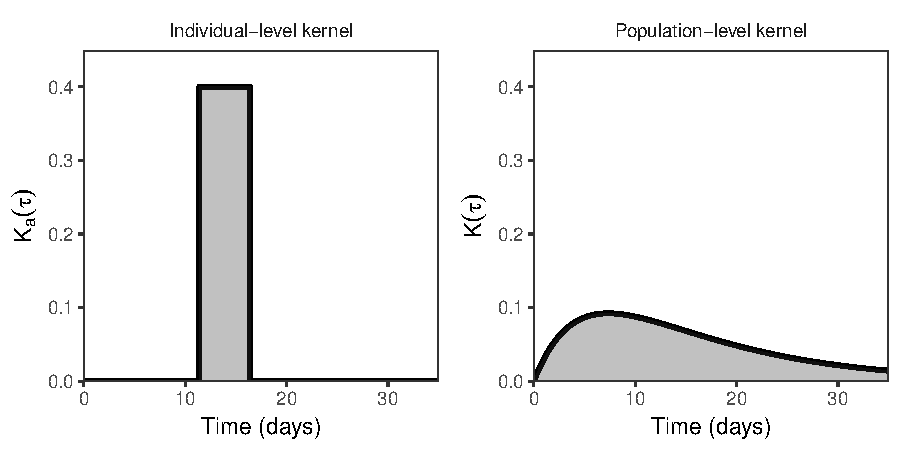
\includegraphics[width=\textwidth]{../fig/individual_and_population.pdf}
\caption{\textbf{Comparison of individual- and population-level kernels.}
(Left) an individual-level kernel of an infected individual with latent period of 11.4 days followed by infectious period of 5 days. 
(Right) a population-level kernel of infected individuals with latent and infectious periods exponentially distributed with means of 11.4 and 5 days, respectively. 
Shaded areas under the curves are equal to individual- and population-level reproductive numbers, both of which are set to 2 in this example.
}
\label{fig:indpop}

\end{figure}

Generation-interval distributions are often considered as population averages, but we can distinguish population-level distributions from individual-level distributions \citep{svensson2007note, svensson2015influence}; 
making this distinction clear will be particularly useful when we discuss spatial components (see \fref{indpop}).
An individual-level intrinsic kernel $K_a(\tau)$ describes the rate at which secondary infections are expected to be caused by an infected individual $a$.
Individuals may vary in their prognosis (e.g., duration of a latent and an infectious period) and their infectiousness, which can depend both on the infectiousness of a disesase as well as the contact structure around them.

The population-level kernel is given by integrating over these individual variations:
\begin{equation}
K(\tau) = \int K_a (\tau) dA.
\end{equation}
The population-level kernel describes the rate at which secondary infections are expected to be caused by an \emph{average} infected individual.
Here, we assume that the individual properties are independent of risk of infection.
In practice, it is unlikely that naively averaging across an empirical distribution will correspond to the correct population-level kernel at a particular time, especially when an epidemic is driven by a few highly infectious individuals. 
\jd{I'd rather drop that clause here; we can get back to it in Discussion if necessary.}

There are two components to an infection kernel: intrinsic infectiousness of an infected individual (the basic reproductive number) and time distribution of new infections (generation-interval distribution).
Assuming that a population mixes homogeneously, we can write: 
\begin{equation}
K(\tau) = \RR_0 g(\tau),
\end{equation}
where $\RR_0 = \int K(\tau) d\tau$ is the basic reproductive number (the expected number of secondary cases caused by an \emph{average} primary case in a fully susceptible population), 
and $g(\tau)$ is the intrinsic generation-interval distribution.

In a homogeneously mixing population, disease incidence $i(t)$ is the product of the current infectiousness of infected individuals and the proportion of the population susceptible, $S(t)$.
\begin{equation}
i(t) = S(t) \int K(s) i(t-s) ds = \RR \int g(s) i(t-s) ds,
\end{equation}
where $\RR = S(t) \RR_0$ is the effective reproductive number.
This model, also referred to as the renewal equation, can represent a wide range of epidemic models \citep{heesterbeek1996concept, diekmann2000mathematical, roberts2004modelling, aldis2005integral, wallinga2007generation, roberts2007model}.
Over a period of time where the proportion of susceptible $S$ remains roughly constant, we would expect approximately exponential growth in incidence $i(t)$; assuming $i(t) = i(0) \exp(r t)$ yields the Euler-Lotka equation \citep{lotka1907relation}, which provides a direct link between speed and strength of an epidemic:
\begin{equation}
\frac{1}{\RR} = \int g(s) \exp(-r s) ds.
\end{equation}

\section{Generation-interval distributions across time}

%% \dc{you make several assertions that are difficult to understand that early in the text. It really doesn't flow well, it was hard to follow, evn fo me who has worked on this kind of things. I suggest you define first c_t.}
%% \jd{I think that verbal explanations first are better for a larger fraction of people. Maybe we can just make the verbal explanations better. I agree that we should keep the horrible math if DC likes it.}

When generation intervals are estimated through contact tracing during an outbreak, infection events that have not happened yet are not observed. 
This effect is called ``right-censoring''.
We can understand the effect of right-censoring using backward generation-interval distributions \citep{tomba2010some, nishiura2010time, champredon2015intrinsic, britton2019estimation}:
the observed (censored) generation-interval distribution is a weighted average of backward generation-interval distributions up until the observation time.

%% \dc{You define $c_t$ after saying this, this is confusing.}
%% During the exponential growth phase, we expect the backward distributions to be the same (and thus the censored distribution should match them). \dc{again, this is explained after... reading doesn't flow well}
%% This connection will break down as the epidemic progresses, however, so we will to distinguish the censored distribution from the backward distribution.

The density of new infections occuring at time $t$ caused by infectors who were infected at time $t-\tau$ is given by
\begin{equation}
i_{t-\tau}(t) = \RR i(t-\tau) g(\tau) S(t)
\end{equation}
The backward generation-interval distribution, $b_t(\tau)$, describes a distribution of infection that occured $\tau$ time units before the referece time $t$ and is proportional to $i(t-\tau) g(\tau)$:
\begin{equation}
b_t(\tau) = \frac{i(t-\tau) g(\tau)}{\int_0^t i(t-\sigma) g(\sigma) d\sigma}
\end{equation}
On the other hand, the censored generation-interval distribution, $c_t(\tau)$, describes a distribution of \emph{all} infections ($i_{s-\tau}(s)$) that are $\tau$ time units apart from any cohort infection time $s$ before $t$.
Then, the censored generation-interval distribution is given by
\begin{equation}\label{eq:obsg}
\begin{aligned}
c_t(\tau) 
&= \frac{\int_0^t i_{s-\tau}(s) ds}{\int_0^t \int_0^t i_{s-\sigma}(s) ds d\sigma}= \frac{\int_0^t i(s-\tau) g(\tau) S(s) ds}{\int_0^t \int_0^t i(s-\sigma) g(x) S(s) ds d\sigma}\\
\end{aligned}
\end{equation}
Substituting $b_s(\tau) = i(s-\tau) g(\tau)$ allows us to rewrite the censored generation-interval distribution as a weighted distribution of the backward generation intervals:
\begin{equation}
c_t(\tau) \propto \int_0^t b_s(\tau) S(s) ds.
\end{equation}
This relationship shows that the backward generation-interval distribution is equivalent to the censored generation-interval distribution when $S \approx 1$, i.e., when the epidemic is growing exponentially.

\begin{figure}[!pbth]
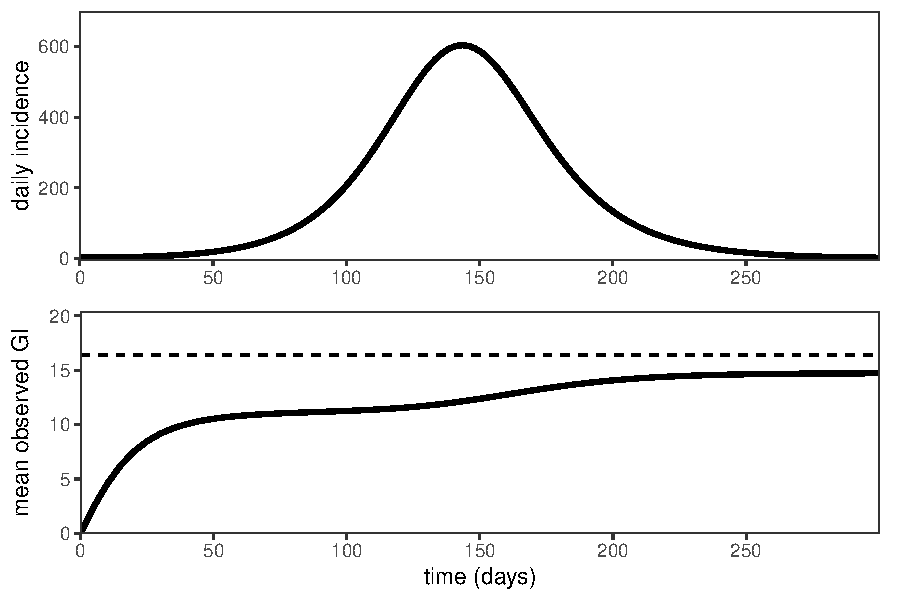
\includegraphics[width=\textwidth]{../fig/temporal_effect.pdf}
\caption{\textbf{Temporal variation in the mean observed generation interval.}
A deterministic Susceptible-Exposed-Infectious-Recovered (SEIR) model was simulated using Ebola-like parameters. The backward and the censored mean generation interval were calculated over the course of an epidemic.
The dotted horizontal line represents the mean intrinsic generation interval.
}
\label{fig:censor}
\end{figure}

For a single epidemic, the observed mean generation interval through contact tracing will always be shorter than intrinsic mean generation interval (Figure~\ref{fig:censor}).
There are two reasons for this phenomenon.
First, any infection events that occur after the contact tracing period cannot be observed due to right censoring and short generation intervals are more likely to be observed.
In particular, when an epidemic is growing exponentially ($i(t) = i(0) \exp(rt)$), 
the censored generation-interval distribution is equivalent to the inverse exponentially weighted intrinsic generation-interval distribution \citep{britton2019estimation}:
\dc{notation $c_{exp}$ is not really consistent with Equation (9) $c_t$}
\jd{Use math formatting in comments or it can mess up the whole doc.}
\begin{equation}
\tsub{c}{exp}(\tau) \propto g(\tau) \exp(-r\tau).
\label{eq:exp}
\end{equation}
During this period, the censored generation-interval distribution has the same mean as the backward generation-interval distribution.
Second, decreasing number of susceptibles over the course of an epidemic makes long infections less likely to occur, and the realized intervals will always be shorter \citep{champredon2015intrinsic}.
As a result, even if contact tracing is performed through an entire epidemic, the mean intrinsic generation interval will be underestimated.
Long backward generation intervals near the end of an epidemic have little effect on the censored generation-interval distributions because they represent only a small portion of an outbreak.

% When a disease is at (or near) endemic equilibrium, the number of susceptibles remains (approximately) constant over time, and we expect the observed generation-interval distribution to be similar to the intrinsic generation-interval distribution.

\section{Generation-interval distributions across space}

Infected individuals may contact the same susceptible individual multiple times, but only the first effective contact gives rise to infection in a given individual (after this, they are no longer susceptible).
Therefore, we expect realized generation intervals to be shorter than intrinsic generation intervals, on average, in a limited contact network.

To explore the effect of multiple contacts on realized generation intervals, we first consider the infection process from an ``egocentric'' point of view, taking into account infectious contacts made by a single infector.
We define the egocentric kernel as the rate at which secondary infections are realized by a single primary case $a$ in the absence of other infectors:
\begin{equation}
\hat{K}_a(\tau) = K_a(\tau) \exp \left(- \delta_a \int_0^\tau K_a(s) ds\right),
\end{equation}
where $K_a(\tau)$ is the individual-level intrinsic kernel and $e^{- \delta_a \int_0^\tau K_a(s) ds}$ is the probability that a susceptible acquaintance has not yet been contacted by individual $a$.
The dilution term, $\delta_a$, models how contacts are distributed among susceptible acquaintances.

Throughout this paper, we assume that there is a constant per-pair contact rate $\lambda$ \citep{trapman2016inferring}.
In this case, the infectiousness of an individual $\RR_a = \int K_a(s) ds$ is the product of the number of acquaintances $N_a$ and the contact rate $\lambda$; the dilution term is equal to the reciprocal of the number of acquaintances: $\delta_a = 1/N_a$.
This assumption can be relaxed by allowing for asymmetry \citep{trapman2016inferring} or heterogeneity \citep{ball1997epidemics, ball2002general} in contact rates; 
for brevity, we do not pursue these directions here.

The population-level egocentric kernel is found by integrating over individual variations:
\begin{equation}\label{eq:ego}
\hat{K}(\tau) = \int \hat{K}_a(\tau) dA.
\end{equation}
\citep{trapman2016inferring} used this same kernel (also assuming a constant per-pair contact rate) to study the effect of network structure on the estimate of reproductive number.
The population-level egocentric generation-interval distribution is:
\begin{equation}
\hat{g}(\tau) = \frac{\hat{K}(\tau)}{\int \hat{K}(s) ds}.
\label{eq:conditional}
\end{equation}
The population-level egocentric generation-interval distribution describes the distribution of times at which secondary infections are realized by an \emph{average} primary case; for convenience, we will often omit ``population-level''.
Finally, the egocentric reproductive number can be estimated by integrating over the egocentric kernel $\hat{K}(\tau)$ directly or by applying the Euler-Lotka equation to the egocentric generation-interval distribution \citep{trapman2016inferring}:
\begin{equation}
\frac{1}{\hat{\RR}} = \int \hat{g}(\tau) \exp(-r \tau) d\tau.
\end{equation}
As the egocentric distribution always has a shorter mean than the intrinsic distribution, \Rhat\ will always be smaller than $\RR$ estimated from the intrinsic distribution;
this generation-interval-based argument provides a clear biological interpretation for the same result presented by \cite{trapman2016inferring}.
% Similarly, \Rhat\ will be greater than the \emph{true} reproductive number \RR\, since it does not account for depletion of susceptibles by other routes.

For example, consider a susceptible-exposed-infected-recovered (SEIR) model, which assumes that latent and infectious periods are exponentially distributed.
The intrinsic generation-interval distribution that corresponds to this model can be written has \citep{svensson2015influence}:
\begin{equation}
g(\tau) = \frac{\sigma \gamma}{\sigma - \gamma} \left(e^{-\gamma t} - e^{-\sigma t}\right),
\end{equation}
where $1/\sigma$ and $1/\gamma$ are mean latent and infectious periods, respectively.
Assuming a constant per-pair contact rate of $\lambda$ for any pair, we obtain the following egocentric generation-interval distribution:
\begin{equation}
\hat{g}(\tau) = \frac{\sigma (\gamma + \lambda)}{\sigma - (\gamma + \lambda)} \left(e^{-(\gamma + \lambda)t} - e^{-\sigma t}\right)
\end{equation}

\dc{I'm surely missing something obvious, but how do you justify this equation from the one above? }

In this case, with fixed infectiousness during the infection period, the effect of accounting for pairwise contacts is the same as an increase in the recovery rate: infecting a susceptible contact is analogous to no longer being infectious (since the contact cannot be infected again). 

This calculation can be validated by simulating stochastic infection processes on a ``star'' network (i.e, a single infected individual at the center connected to multiple susceptible individuals who are not connected with each other).
Simulations confirm that in this case the distribution of \emph{contact} times matches the intrinsic generation-interval distribution, while the distribution of realized generation times (i.e., \emph{infection} times) matches the egocentric generation-interval distribution (\fref{local}).

\jd{I want to keep thinking about network choice. Would a random network be useful? Are we careful enough about time windows (exponential phase vs (roughly) full single epidemic?}
\begin{figure}[!pbth]
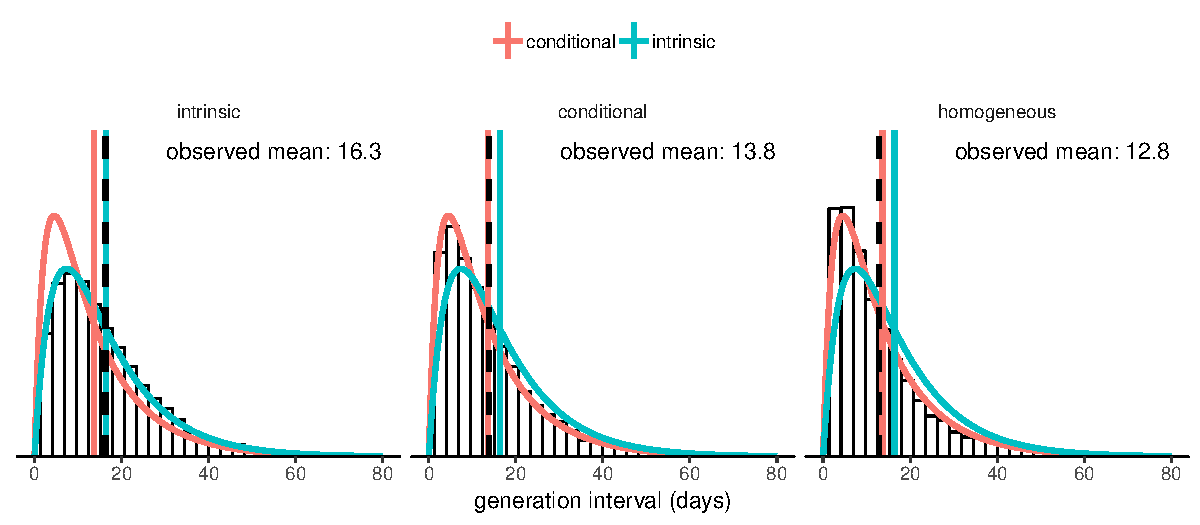
\includegraphics[width=\textwidth]{../fig/local_effect.pdf}
\caption{
\textbf{Spatial effects on realized generation intervals.}
Theoretical distributions and means are shown in color (and are the same in each panel, for reference). Simulated distributions and means are shown in black.
(Left) the intrinsic generation-interval distribution corresponds to all contacts by a focal individual, regardless of whether the individual contacted is susceptible (simulated on a star network).
(Middle) the egocentric generation-interval distribution corresponds to the distribution of all infectious contacts by the focal individual with susceptible individuals, in the case where the focal individual is the only possible infector (simulated on a star network).
(Right) realized generation-interval distributions are shorter than egocentric distributions in general, because contacts can be wasted when susceptibles become infected through other routes (simulated on a homogeneous network).
All figures were generated using 5000 stochastic simulations on a network with 5 nodes (1 infector and 4 susceptibles).
}
\label{fig:local}
\end{figure}

The egocentric generation interval \eref{conditional} only explains some of the reduction in generation times that occurs on most networks, however.
Generation intervals are also shortened by indirect connections: a susceptible individual can be infected through another route before the focal individual makes infectious contacts.
Simulations on a small homogeneous network confirm this additional effect (\fref{local}, right panel). 

In general, spatial reduction in the mean generation interval can be viewed as an effect of susceptible depletion and can be further classified into three levels: egocentric, local, and global.
Egocentric depletion, as discussed previously, is caused by an infected individual making multiple contacts to the same individual.
Local depletion refers to a depletion of susceptible individuals in a household or neighborhood;
this effect can be observed early in an epidemic, especially in a highly structured population, even if most of the population remains susceptible.
Finally, global depletion refers to overall depeletion of susceptibility as a population-level and explains the reduction in realized compared to intrinsic generation intervals that occurs even in a well-mixed population (\fref{censor}). 
\dc{Would it be possible to define local depletion using a more rigorous network topology, rather than households/neighborhood? (Would it help?). The same way the egocentric is defined with a star-shaped network, can we define the local depletion with a (well-known?) shape? Global depletion may be fine as it is, as this is something we are used to in general (in other modelling frameworks). }

\section{Inferring generation-interval distributions from a contact tracing data}

When generation intervals are sampled through contact tracing, there will be four effects present in the sample: (1) right-censoring effect, (2) egocentric depletion effect, (3) local depletion effect and (4) global depletion effect.
We can correct explicitly for the egocentric effect and, in the case of exponential growth, the right-censoring effect.
While the other two effects are difficult to measure, we can make qualitative predictions about their effects on the realized generation intervals and reproductive numbers: 
both local and global depletion effects reduce number of infections that occur and shorten generation intervals.
% SWP: I would rather put these in Discussion?
% but the time scale on which they matter differs:
% local depletion will be important early in an epidemic whereas global depletion will be small until sufficient amount of susceptible individuals become infected.
% As a result, we expect the initial spread of a disease and the realized reproductive number to be heavily dependent on local structure of the contact network near the source of an outbreak.

Since the right-censoring effect is a sampling bias, we want to take it into account explicitly.
In contrast, spatial effects have the same effect on how the epidemic spreads as they do on observed generation intervals. 
We therefore expect that if we correct observed generation intervals for the right-censoring effect, spatial components will be taken into account implicitly. 
We can use these temporally corrected intervals to correctly link $r$ and $\RR$.
Hereafter, we will refer to the temporally corrected distribution as the ``effective'' generation-interval distribution. 
The effective distribution incorporates spatial effects. 
In a large homogeneously mixing population, the effective distribution will be equivalent to the intrinsic distribution.

\begin{figure}[!pbth]
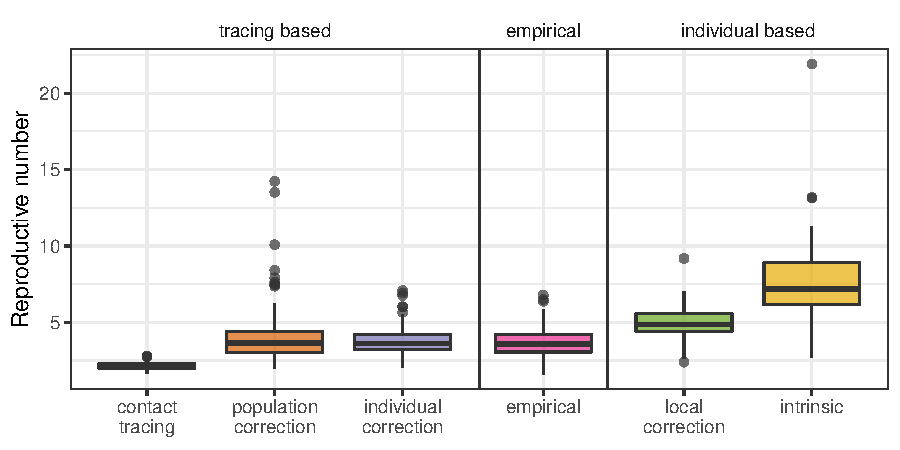
\includegraphics[width=\textwidth]{../fig/cmp_reproductive.pdf}
\caption{\textbf{Comparison of estimates of reproductive number based on various methods.}
Using the observed generation-interval distributions without correcting for right-censoring severely underestimates the reproductive number.
Similarly, using intrinsic and egocentric generation-interval distributions without accounting for local spatial effects overestimates the reproductive number.
Both population-level and individual-level methods provide estimates of reproductive number that are consistent with the empirical estimates, which we define as the average number of secondary cases generated by the first 100 infected individuals.
Boxplots are generated using 100 stochastic simulations of the SEIR model on an empirical network using Ebola-like parameters.
}
\label{fig:cmp}
\end{figure}

Here, we investigate two methods for correcting for temporal bias in a contact tracing data.
We refer to the first method as the population-level method as it relies on the observed distribution aggregated across the entire population.
As the observed generation-interval distribution is a weighted distribution of the effective distribution, the effective distribution can be recovered by taking the inverse of the weights, given by \eref{exp}.
Hence, the population-level method relies on the observed generation intervals and the exponential growth rate \citep{tomba2010some, nishiura2010time, britton2019estimation}:
\begin{equation}
g(\tau) \propto \tsub{c}{exp}(\tau) \exp(r\tau).
\end{equation}
When the susceptible dynamics is known, this equation can be generalized by using \eref{obsg}; we do not pursue this direction here.
The population-level method is simple and intuitive, but does not take into account who infected whom.

We refer to the second method as the individual-level method because it relies on individual contact information.
We model each infection $i$ from an infected individual $j$ as a non-homogeneous Poisson process between the time at which infector $j$ was infected ($t_j$) and the censorship time ($\tsub{t}{censor}$), where the time-varying Poisson rate at time $t$ is equal to $\RR g(t - t_j)$, where $g(t)$ is the effective generation-interval distribution \citep{daley2007introduction}.
\dc{is effective GI distribution, $g$, the same as the intrinsic? The notation implies it is... but I'm confused now.}
We use a gamma distribution (parameterized by its mean and shape) to model the effective generation-interval distribution.
Then, the probability that an individual $j$ infects $n_j$ individuals between $t_j$ and $\tsub{t}{censor}$ is equal to
\begin{equation}
\frac{\RR^{n_j} \exp \big(- \RR G(\tsub{t}{censor} - t_j ;\theta) \big) \prod_{i=1}^{n_j} g(s_{i, j}; \theta)}{n_j!},
\end{equation}
where $s_{i,j}$ is the observed generation interval between infector $j$ and infectee $i$, and $\theta$ is a (vector) parameter of the generation-interval distribution $g$ (and the corresponding cumulative distribution function $G$).

The entire data likelihood of the individual-level method can be written as:
\begin{equation}
\begin{aligned}
&\mathcal{L}(\RR, \theta\,|\, \mathbf{s}, \mathbf{t}, \mathbf{n}, \tsub{t}{censor})\\
&\quad=\prod_{j=1}^N \left(\RR^{n_j} \exp \big(- \RR G(\tsub{t}{censor} - t_j ;\theta) \big) \prod_{i=1}^{n_j} g(s_{i, j}; \theta) \right),
\end{aligned}
\end{equation}
where $N$ is the total number of infected individuals.
Here, we estimate parameters $\RR$ and $\theta$ by maximum likelihood.
Since the estimate of $\RR$ is sensitive to under-reporting, we use the estimated generation-interval distribution to infer the effective reproductive number from the estimated growth rate.
\cite{forsberg2008likelihood} proposed a related approach based on discretized incidence reports.

\dc{that reminds me of Cauchemez's 2006 AJE paper: ``Estimating in Real Time the Efficacy of Measures to Control Emerging Communicable''. Not sure if it's really relevant, but just in case...  }

To test these methods, we simulate 100 epidemics with Ebola-like parameters on an empirical network \citep{leskovec2016snap} and compare the estimates of reproductive number with empirical reproductive numbers, which we define as the average number of secondary cases generated by the first 100 infected individuals (\fref{cmp}).
\cite{trapman2016inferring} defined the empirical reproductive number by dividing the total number of infected individuals in generations $2$ to $k+1$ by the total number of infected individuals in generations $1$ to $k$, where the reference generation $k$ is defined to be the first generation that contains at least 75 infected individuals;
however, individuals in later generations are potentially subject to stronger local depletion and even global depletion effects.
Therefore, we expect our empirical estimate to better reflect the infection process during the exponential growth phase.
\swp{TODO: Compare Trapman vs our estimate of empirical R0 in Appendix; Trapman estimate is much lower.}

As we predicted earlier, calculating reproductive number based on the intrinsic generation-interval distribution overestimates the empirical reproductive number;
estimates based on the egocentric generation-interval distribution (\eref{conditional}) are closer to empirical reproductive numbers but still suffer from overestimation as they do not account for indirect spatial effects. \dc{Figure? I guess this is work in progress...}
Direct estimates based on contact tracing data severely underestimates the empirical estimates.
While both population- and individual-level corrections provide similar estimates to the empirical reproductive number,
population-level estimates are more variable as they are more sensitive to outliers in generation intervals and our estimate of the growth rate.
For smaller values of \RR, we expect the differences to become smaller. 
\swp{TODO: In Appendix, we present the same figure using Erlang-distributed latent periods, which better corresponds to Ebola. Overall, our qualitative conclusions do not change.}

\section{Discussion}

The intrinsic generation-interval distribution, which describes the expected time distribution of secondary cases, provides a direct link between speed (exponential growth rate, $r$) and strength (reproductive number, $\RR$) of an epidemic \citep{wallinga2007generation, svensson2007note, svensson2015influence, park2019practical}.
However, observed generation-interval distributions can vary depending on how and when they are measured \citep{nishiura2010time, tomba2010some, champredon2015intrinsic, britton2019estimation};
determining which distribution correctly links $r$ and $\RR$ can be challenging.
Here, we analyze how observed generation intervals, measured through contact tracing, differ from intrinsic generation intervals.
Changes due to temporal censoring reflect observation bias, whereas changes due to spatial or network structure reflect the dynamics of the outbreak.
Thus correcting the observed distribution for temporal, but not spatial, effects provides the correct link between $r$ and $\RR$.

Observed generation intervals are subject to right-censoring -- it is not possible to trace individuals that have not been infected yet.
These right-censored distributions can be thought of as averages of ``backward'' generation intervals (measured by tracing the infectors of a cohort of infected individuals) \citep{kenah2008generation, nishiura2010time, tomba2010some, champredon2015intrinsic, britton2019estimation}.
During an ongoing outbreak, the observed generation-interval distribution will always have a shorter mean than the intrinsic-interval distribution due to right-censoring.
Early in the outbreak, censored intervals are expected to match the early-outbreak backward intervals.
Near the end of an outbreak, the effect of right-censoring becomes negligible but the observed generation intervals are still shorter on average than intrinsic generation intervals, because of depletion of the susceptible population.

We classified susceptible depletion into three levels: egocentric, local, and global.
Egocentric susceptible depletion refers to the effect of an infected individual making multiple contacts to the same susceptible individual.
Accounting for the egocentric effect allowed us to reinterpret the results by \cite{trapman2016inferring} using arguments based on generation intervals.
Local susceptible depletion refers to the effect of other closely related infected individuals (e.g., in a household or neighborhood) making multiple contacts to the same susceptible individual.
Global susceptible depletion refers to the overall decrease in the susceptible pool in the population.

Susceptible depletion happening at all three levels shortens realized generation intervals but acts on different time scales.
Egocentric and local depletion effects are present from the beginning of an epidemic, even when depletion in the global susceptible population is negligible, and can strongly affect the initial spread of an epidemic.
Therefore, we predicted the observed generation intervals during an exponential growth phase to contain information about the contact structure, allowing us to estimate the \emph{effective} generation-interval distribution by simply accounting for the right-censoring.
Simulation studies confirmed our prediction: using the effective generation-interval distribution provides the correct link between $r$ and $\RR$.

We compare two methods for estimating the effective generation-interval distribution and assume that the effective generation-interval distribution follows a gamma distribution.
The gamma approximation of the generation interval distribution has widely used due to its simplicity;
we previously thought that summarizing the entire distribution with two moments (mean and variance) is sufficient to understand the role of generation-interval distributions in linking $r$ and $\RR$.
However, further investigation of our methods suggests that making a wrong distributional assumption leads to overly narrow confidence intervals, even though the gamma distribution looks indistinguishable from the shape of the intrinsic generation-interval distribution (derived from the SEIR model) \swp{Appendix}.
These results are particularly alarming because it is impossible to know the true shape of the distribution [CITE].

The generation-interval-based approach to estimating the reproductive number assumes that an epidemic grows exponentially \citep{wallinga2007generation, park2019practical}.
In practice, heterogeneity in population structure can lead to subexponential growth \citep{szendroi2004polynomial, chowell2015western, chowell2016growing, chowell2016characterizing, kiskowski2016modeling, viboud2016generalized};
we therefore expect our simulations on an empirical network to be better characterized by subexponential growth models \citep{viboud2016generalized}.
However, our simulations suggest that the initial exponential growth assumption still provides a viable approach for estimating the reproductive number.
This conclusion is supported by \cite{chowell2015western} who found that epidemics can exhibit exponential growth patterns globally even if local epidemics may not.


\swp{Conclusion?}
\jd{Let me try.}

\section{Methods}

\subsection{Deterministic SEIR model}

\swp{CITE}
To study the effects on right-censoring on the observed generation intervals, we use the deterministic Susceptible-Exposed-Infectious-Recovered (SEIR) model.
The SEIR model describes how a disease spreads in a homogeneously mixing population; it assumes that infeceted individuals become infectious after a latent period.
We use a \seminar\ model, which extends the SEIR model to have multiple equivalent stages in the latent and infectious periods. This gives periods with Erlang distributions (gamma distributions with integer shape parameters), which are often more realistic than the exponentially distributed periods in the standard SEIR model: 
\jd{Mention that our main-text models use exponential later instead.}
\begin{equation}
\begin{aligned}
\frac{dS}{dt} &= - \beta S \frac{\sum_{k=1}^{n_I} I_k}{N}\\
\frac{dE_1}{dt} &= \beta S \frac{\sum_{k=1}^{n_I} I_k}{N} - n_E \sigma E_1\\
\frac{dE_m}{dt} &= n_E \sigma (E_{m-1} - E_m) && \text{for } m = 2, 3, \dots, n_E\\
\frac{dI_1}{dt} &= n_E \sigma E_m - n_I \gamma I_1\\
\frac{dI_n}{dt} &= n_I \gamma (I_{n-1} I_n) && \text{for } n = 2, 3, \dots, n_I\\
\end{aligned}
\end{equation}
where $S$ is the number of susceptible individuals, $E_m$ is the number of exposed individuals in the $m$-th compartment, $I_n$ is the number of infectious individuals in the $n$-th compartment, and $R$ is the number of recovered individuals.
Parameters of the model are specified as follows: $N$ is the total population size, $\beta$ is the transmission rate, $1/\sigma$ is the mean latent period, and $1/\gamma$ is the mean infectious period.

\subsection{Stochastic SEIR model}

\swp{What do I cite here?}
We develop an algorithm to simulate an individual-based SEIR model on a network to keep track of generation intervals.
Our algorithm is based on the Gillespie algorithm.
We model individuals with nodes on a network and their acquaintanceships with edges; infected individuals can only contact their acquaintances.

First, we begin by randomly selecting initially infected individuals; these individuals are assumed to be infected at $t = 0$.
For each infected individual $i$, we randomly draw the latent period $E_i$ from an Erlang distribution with mean $1/\sigma$ and shape $n_E$.
We then construct the random infectious period and infectious contact times simultaneously as follows.
For each of the $n_I$ stages of the infectious period, we draw the number of effective contacts from a geometric distribution with mean $S_i \lambda / n_I\gamma$, where $S_i$ is the number
of susceptible acquaintances and $\lambda$ is the per-pair contact rate.
We then choose the time between consecutive events (the chosen number of contacts, followed by exit from the given stage of infection) from an exponential distribution with rate $S_i \lambda + n_I\gamma$.
For each contact, a contactee is uniformly sampled from the set of susceptible acquaintances of the individual $i$.
The infectious period $I_i$ is the sum of all of these waiting times.

[[Add flowchart?]]

After repeating the contact process for all initially infected individuals, all contacts are put into a sorted queue.
The first person in the queue becomes infected, and the current time is updated to infection time of this individual. 
Any subsequent contacts made to this individual are removed from the queue because they will no longer be effective.
We repeat the contact process for this newly infected individual.
Then, new contacts are added to the sorted queue.
The simulation continues until there are no more contacts are left in the queue.

\subsection{Empirical network}

To simulate epidemics on a realistic network, we use the `condensed matter physics' network from the Stanford Large Network Dataset Collection \citep{leskovec2016snap}.
This graph describes co-authorship among anyone who submitted a paper to Condensed Matter category in the arXiv between January 1993 and April 2003 \citep{leskovec2007graph}.
It consists of 23133 nodes and 93497 edges.
\cite{trapman2016inferring} used the same network to simulate epidemics.

\subsection{Measuring the exponential growth rate}

We estimate the exponential growth rate $r$ of an epidemic from daily incidence by modeling the cumulative incidence $c(t)$ with a logistic function \citep{ma2014estimating}: 
\begin{equation}
c(t) = \frac{K}{1 + \left[(K/c_0) - 1\right] e^{-rt}},
\end{equation}
where $K$ is the final size of an epidemic and $c_0$ is the initial number of cases.
Fitting this curve directly to cumulative incidence can lead to overly confident result \citep{king2015avoidable}; instead we fit interval incidence $x(t) = c(t + \Delta t) - c(t)$, where $\Delta t$ is 1 day, to daily incidence, assuming that daily incidence follows a negative binomial distribution. 
This assumption requires us to estimate the dispersion parameter $\theta$ of a negative binomial distribution.
Parameters $r$, $K$, $c_0$, and $\theta$ are estimated simultaneously by maximizing the likelihood.


\section{Appendix}

\bibliography{network}
\end{document}
